\section{Verifiable Research-Loop}
\label{sec:method}

Given a workspace containing read-only input data (\texttt{data/}), generated analysis scripts (\texttt{code/}), raw execution stdout logs (\texttt{out/}), and a drafted report (\texttt{report/report.md}), Verifiable Research-Loop decides whether the deliverable may be released or must return for targeted repair.
Figure~\ref{fig:arch} contrasts our two-layer architecture against bare execution (\texttt{B0}), existence gating (\texttt{B1}), and advisory cross-model review (\texttt{B2}).
The harness couples three deterministic pre-audit modules with a path-isolated cross-family auditor and a persistent USD budget circuit breaker, built entirely on the Python standard library.

\begin{figure*}[t]
  \centering
  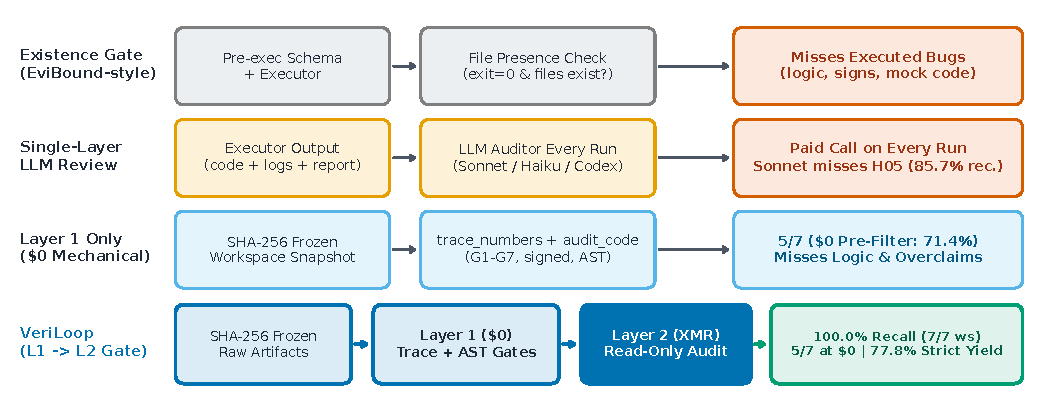
\includegraphics[width=\textwidth]{figures/fig1_architecture.pdf}
  \caption{\textbf{Dual-layer hard gating closes the verification gap left by existence checks and advisory review.} Comparison of the four evaluated governance paradigms: bare execution (\texttt{B0}), existence gating (\texttt{B1}, grey), summary-fed advisory cross-model review (\texttt{B2}, amber), and Verifiable Research-Loop (blue). Our harness executes deterministic claim, numerical-provenance, and Python AST gates before path-isolated cross-family auditing, enforcing hard blocking and one-round closed-loop repair (green).}
  \label{fig:arch}
\end{figure*}

\subsection{Pre-Registered Claim Ledger and Hard Gates (\texttt{G1--G7})}
\label{sec:claims}

Unconstrained research agents frequently shift hypotheses after seeing noisy outputs or promote unlogged pilot trials into headline claims.
To bind conclusions to pre-execution intent, \texttt{claims.py} records every candidate claim before experiments run, specifying an immutable falsification criterion, primary metric, and dataset scope.
Every claim enters the ledger in \texttt{pilot} state and cannot be promoted to \texttt{supported} unless seven deterministic gates pass (formal specifications in Appendix~\ref{app:gates}):
\texttt{G1} verifies log file presence, intact SHA-256 digests against post-hoc tampering, and explicit completion markers against truncated runs;
\texttt{G2} enforces per-dataset and per-arm multi-seed floors (or explicit deterministic registration);
\texttt{G3} and \texttt{G4} enforce validation-only hyperparameter tuning and pre-registered baseline comparisons;
\texttt{G5} requires dedicated ablation log files rather than prose assertions;
\texttt{G6} assigns strictly monotonic sequence counters and microsecond ISO timestamps to prevent retroactive ledger edits; and
\texttt{G7} verifies machine-parseable uncertainty intervals ($\pm$ or $[l,u]$) or $p$-values inside linked logs.
This fail-closed design guarantees that any unverified claim remains \texttt{unsupported} unless explicitly waived by a human researcher.

\subsection{Deterministic Numerical Provenance and Static AST Gates}
\label{sec:mech_gates}

Even when an agent registers claims and executes scripts cleanly, \textsc{FabScore}~\citep{chen2026fabscore} shows that 85.9\% of result fabrications contradict existing logs and 44.6\% of experiment fabrications involve hardcoded or mocked code.
Our second deterministic layer inspects both reported numbers and source code at zero LLM cost before invoking any external reviewer.

\paragraph{Signed numerical provenance (\texttt{trace\_numbers.py} v2).}
The tracer indexes every floating-point token across \texttt{out/} and \texttt{outputs/}, preserving sign, decimal precision, and line co-occurrence, and checks every decimal with at least three decimal places in \texttt{report/report.md}.
It enforces four hard invariants:
(1) \texttt{SIGN\_MISMATCH} catches sign-flip fabrications where a negative logged delta is reported as positive while normalizing Unicode minus (\texttt{U+2212}), ASCII \texttt{+/-} spacing, spaced binary subtraction, and trailing-zero equality (\texttt{1.000} vs.\ \texttt{1.0});
(2) \texttt{WRONG\_LOG} requires every number on a table row citing a log filename to appear inside that exact log rather than elsewhere in the workspace;
(3) \texttt{UNPAIRED\_PM/CI} verifies that \texttt{mean$\pm$std} and \texttt{[lo, hi]} bounds co-occur on the same raw log line; and
(4) \texttt{CITED\_STALE} flags logs older than the scripts that generated them.

\paragraph{Static Python AST integrity (\texttt{audit\_code.py}).}
To catch code-level shortcuts invisible to output existence checks, \texttt{audit\_code.py} parses every Python script in \texttt{code/} using stdlib \texttt{ast} and detects six high-risk patterns:
\texttt{HARDCODED\_REF\_PRINT} (printing literal reference scores instead of computing them),
\texttt{HARDCODED\_METRIC\_ARRAY},
\texttt{MOCK\_FALLBACK} (substituting random or synthetic data when files are missing or empty),
\texttt{TEST\_TUNING} (selecting checkpoints or hyperparameters using test-split variables),
\texttt{OPTIMISTIC\_TIE} (strict-greater ranking tie bugs), and
\texttt{DEAD\_METRIC} (defined but uncalled metric functions), alongside report scope-overclaim markers.
Any \texttt{HIGH}-severity AST finding or numerical tracing error triggers an immediate hard delivery block.

\subsection{Path-Isolated Cross-Family Auditing and Closed-Loop Repair}
\label{sec:xmr}

Deterministic gates catch syntactic, cryptographic, and numerical mismatches cleanly, yet they cannot judge whether a valid-looking script implements a flawed statistical denominator or overstates an observational correlation as causation.
To detect semantic and methodological fabrications without inheriting the executor's blind spots, \texttt{run\_audit.py} invokes an independent auditor from a distinct model family inside a strictly read-only sandbox.

Crucially, the auditor never receives the executor's narrative summary, reasoning chain, or self-assessment.
Its prompt contains only raw filesystem paths (\texttt{data/}, \texttt{code/}, \texttt{out/}, \texttt{report/report.md}), the deterministic pre-audit JSON, and a 38-item hostile checklist covering provenance, baselines, selection, matched comparisons, attribution, statistics, measurement, scope, trajectory, and code integrity.
The auditor reads raw CSVs, scripts, and logs directly, recomputes suspicious statistics read-only, and emits line-cited findings plus a structured JSON verdict (Appendix~\ref{app:gates}) separating valid work (\texttt{APPROVE\_SUPPORTED}), honest refusal (\texttt{APPROVE\_HONEST\_REFUSAL}), publication-sufficiency gaps (\texttt{BLOCK\_UNSUPPORTED}), and scientific misconduct or calculation errors (\texttt{BLOCK\_MISCONDUCT}).

Any mechanical gate failure or \texttt{BLOCK\_*} verdict halts delivery deterministically.
When closed-loop revision is enabled (\texttt{--max-revisions 1}), the harness snapshots the blocked report, returns only the mechanical error list and \texttt{audits/01-review.md} to the executor for one repair turn, and then runs a fresh Round-2 deterministic pre-audit and cross-family review (\texttt{audits/02-review.md}).
A persistent USD ledger (\texttt{budget.py}) enforces a hard cost circuit breaker before every LLM call so automated verification loops never exceed their compute budget.
